\documentclass[aspectratio=169, 10pt]{beamer}

% --- Theme & Styling ---
\usetheme{metropolis}
\usepackage{booktabs}
\usepackage{xspace}
\usepackage{tikz}
\usetikzlibrary{arrows.meta, positioning, shapes.geometric, calc}
\usepackage{listings}
\usepackage{tcolorbox}
\usepackage{graphicx}
\usepackage{caption}

% Caption styling for epigraphs below figures
\captionsetup{font=scriptsize, labelfont=bf, textfont=it, skip=2pt, justification=centering}

% --- Color Palette ---
\definecolor{NavyDark}{HTML}{0F172A}
\definecolor{PrimaryBlue}{HTML}{1D4ED8}
\definecolor{TealDark}{HTML}{0F766E}
\definecolor{AmberWarm}{HTML}{B45309}
\definecolor{BgSlate}{HTML}{F8FAFC}
\definecolor{CodeSlate}{HTML}{1E293B}

\setbeamercolor{normal text}{fg=NavyDark, bg=white}
\setbeamercolor{alerted text}{fg=AmberWarm}
\setbeamercolor{example text}{fg=TealDark}
\setbeamercolor{progress bar}{fg=PrimaryBlue, bg=gray!25}
\setbeamercolor{title separator}{fg=PrimaryBlue}
\setbeamercolor{frametitle}{bg=NavyDark, fg=white}

% Metropolis tuning
\metroset{progressbar=frametitle, block=fill}

% Custom image frame styling for screenshots
\newtcbox{\imageframe}{
    colback=NavyDark,
    colframe=NavyDark!40!gray,
    arc=0mm,
    boxrule=0.6pt,
    left=1pt,
    right=1pt,
    top=1pt,
    bottom=1pt,
    boxsep=0pt,
    nobeforeafter
}

% --- Title Information ---
\title{Lab 2: 64-Bit XGMII Interface \& Reconciliation Sublayer}
\subtitle{Hardware-in-the-Loop Simulation, FCS CRC-32 \& 64-Bit Waveform Analysis}
\date{\today}
\author{Zuñiga, Ivan Andrés}
\institute{Fundación Fulgor}

\begin{document}

% ==========================================
% SLIDE 1: Title Slide
% ==========================================
\maketitle

% ==========================================
% SLIDE 2: Testbench Architecture & Pipeline
% ==========================================
\begin{frame}{1. System Architecture \& 64-Bit XGMII Datapath}
\vspace{1mm}
\begin{columns}[c]
    \begin{column}{0.48\textwidth}
        \textbf{Hardware-in-the-Loop Setup:}
        \begin{itemize}\small
            \item \textbf{Host Interface}: \texttt{tap0} (\texttt{10.0.0.1/24}, MAC \texttt{02:00:00:00:00:01}).
            \item \textbf{Target Interface}: \texttt{tap1} in namespace \texttt{ns\_b} (\texttt{10.0.0.2/24}, MAC \texttt{02:00:00:00:00:02}).
            \item \textbf{C++ Testbench (\texttt{wrapper.cpp})}: Non-blocking TAP I/O, converts L2 frames to 64-bit XGMII SDR words, appends IEEE 802.3 CRC-32 FCS, and checks FCS on RX.
            \item \textbf{RTL Core (\texttt{top.sv})}: Synchronous 8-lane parallel datapath (\texttt{txd[63:0]}, \texttt{txc[7:0]}) with FSM header extraction and sliding-window FCS latching.
            \item \textbf{Standard}: IEEE 802.3 Clause 81 Reconciliation Sublayer (64-bit SDR MII mapping with \texttt{/S/}, \texttt{/T/}, and \texttt{/I/}).
        \end{itemize}
    \end{column}
    
    \begin{column}{0.50\textwidth}
        \begin{tcolorbox}[colback=BgSlate, colframe=PrimaryBlue, title=\footnotesize 64-Bit XGMII Simulation Architecture, arc=2mm, top=1.5mm, bottom=1.5mm]
            \centering
            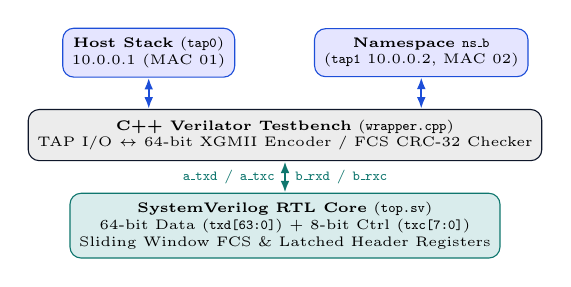
\begin{tikzpicture}[node distance=0.55cm, every node/.style={font=\tiny, align=center}]
                \node[draw=PrimaryBlue, fill=blue!10, rounded corners, minimum width=2.0cm, minimum height=0.6cm] (host) {\textbf{Host Stack} (\texttt{tap0})\\10.0.0.1 (MAC 01)};
                \node[draw=PrimaryBlue, fill=blue!10, rounded corners, minimum width=2.0cm, minimum height=0.6cm, right=1.0cm of host] (nsb) {\textbf{Namespace \texttt{ns\_b}}\\(\texttt{tap1} 10.0.0.2, MAC 02)};
                
                \node[draw=NavyDark, fill=gray!15, rounded corners, minimum width=4.4cm, minimum height=0.65cm, below=0.4cm of $(host.south)!0.5!(nsb.south)$] (wrap) {\textbf{C++ Verilator Testbench} (\texttt{wrapper.cpp})\\TAP I/O $\leftrightarrow$ 64-bit XGMII Encoder / FCS CRC-32 Checker};
                
                \node[draw=TealDark, fill=teal!15, rounded corners, minimum width=4.4cm, minimum height=0.65cm, below=0.4cm of wrap] (rtl) {\textbf{SystemVerilog RTL Core} (\texttt{top.sv})\\64-bit Data (\texttt{txd[63:0]}) + 8-bit Ctrl (\texttt{txc[7:0]})\\Sliding Window FCS \& Latched Header Registers};
                
                % Arrows
                \draw[{Latex[length=1.5mm]}-{Latex[length=1.5mm]}, thick, color=PrimaryBlue] (host) -- (host |- wrap.north);
                \draw[{Latex[length=1.5mm]}-{Latex[length=1.5mm]}, thick, color=PrimaryBlue] (nsb) -- (nsb |- wrap.north);
                \draw[{Latex[length=1.5mm]}-{Latex[length=1.5mm]}, thick, color=TealDark] (wrap) -- node[left, font=\tiny]{\texttt{a\_txd} / \texttt{a\_txc}} node[right, font=\tiny]{\texttt{b\_rxd} / \texttt{b\_rxc}} (rtl);
            \end{tikzpicture}
        \end{tcolorbox}
        \vspace{1mm}
        \captionof{figure}{Simulation connecting Linux TAP network stacks to the 64-bit XGMII RTL pipeline.}
    \end{column}
\end{columns}
\end{frame}

% ==========================================
% SLIDE 3: Environment Setup & Traffic Generation
% ==========================================
\begin{frame}{2. Environment Setup \& Traffic Generation}
\vspace{1mm}
\begin{columns}[c]
    \begin{column}{0.48\textwidth}
        \textbf{Execution Sequence:}
        \begin{enumerate}\footnotesize
            \item \textbf{TAP Network Initialization}:\\
            \texttt{sudo ./setup\_tap.sh}\\
            {\scriptsize Configures \texttt{tap0} and isolated namespace \texttt{ns\_b} with \texttt{tap1}.}
            
            \item \textbf{Verilator Build \& Execution}:\\
            {\scriptsize\texttt{verilator --cc --trace --exe --build wrapper.cpp top.sv}}\\
            \texttt{sudo ./obj\_dir/emulator}
            
            \item \textbf{Traffic Capture}:\\
            \texttt{sudo tcpdump -i tap0 -w lab2\_capture.pcap}
            
            \item \textbf{Pattern Traffic Injection}:\\
            \texttt{ping -c 2 -p cafe0002 -I tap0 10.0.0.2}
        \end{enumerate}
    \end{column}
    
    \begin{column}{0.50\textwidth}
        \centering
        \imageframe{
\includegraphics[width=0.96\linewidth, height=0.64\textheight, keepaspectratio]{figures/screenshot1_terminal.png}}
        \vspace{1mm}
        \captionof{figure}{Terminal execution: TAP interface binding, Verilator build, and no loss in ICMP traffic.}
    \end{column}
\end{columns}
\end{frame}

% ==========================================
% SLIDE 4: Wireshark Packet Inspection
% ==========================================
\begin{frame}{3. Layer 2 / Layer 3 Wireshark Packet Analysis}
    \vspace{1mm}
    \textbf{Captured ICMP Echo Request Frame (98 Bytes Total):}
    \begin{itemize}\scriptsize
        \item \textbf{Layer 2 Header (14B)}: Dst MAC \texttt{02:00:00:00:00:02}, Src MAC \texttt{02:00:00:00:00:01}, EtherType \texttt{0x0800} (IPv4).
        \item \textbf{Layer 3/4 Header (28B)}: IPv4 \texttt{10.0.0.1} $\rightarrow$ \texttt{10.0.0.2} (20B, Len 84B, ID \texttt{0x7E53}), ICMP Type 8 (Echo Request, Code 0, Checksum \texttt{0xECEC}, ID \texttt{0x4702}, Seq 1).
        \item \textbf{Payload (56B)}: 16-byte kernel timestamp + 40-byte repeating pattern \texttt{ca fe 00 02} (offsets \texttt{0x003a}--\texttt{0x0061}).
    \end{itemize}
    
    \vspace{1mm}
    \begin{center}
        \imageframe{
\includegraphics[width=0.94\textwidth, height=0.45\textheight, keepaspectratio]{figures/screenshot2_wireshark.png}}
        \vspace{1mm}
        \captionof{figure}{Wireshark dissection and hex dump of the 98-byte captured ICMP frame.}
    \end{center}
\end{frame}

% ==========================================
% SLIDE 5: XGMII Start Delimiter & Preamble / SFD
% ==========================================
\begin{frame}{4. XGMII Framing: Frame Start Delimiter \& Preamble}
    \vspace{1mm}
    \textbf{Start Control Character \& Preamble/SFD Lane Alignment (IEEE 802.3 Clause 81):}
    \begin{itemize}\scriptsize
        \item \textbf{Start Delimiter (\texttt{/S/ = 0xFB})}: Aligned to Lane 0 with control bit \texttt{TXC[0] = 1} (\texttt{TXC = 8'h01}).
        \item \textbf{Preamble \& SFD Sequence}: 6 Preamble bytes (\texttt{0x55}) on Lanes 1--6, followed by 1 SFD byte (\texttt{0xD5}) on Lane 7 (\texttt{TXD = 0xD5555555555555FB}).
    \end{itemize}
    
    \vspace{1mm}
    \begin{center}
        \imageframe{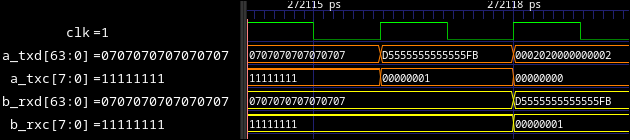
\includegraphics[width=0.94\textwidth, height=0.45\textheight, keepaspectratio]{figures/screenshot3_preamble_start.png}}
        \vspace{1mm}
        \captionof{figure}{Transition from Idles (\texttt{/I/ = 0x07}) to Start of Frame (\texttt{/S/ = 0xFB}) on Lane 0.}
    \end{center}
\end{frame}

% ==========================================
% SLIDE 6: SW-to-HW Correlation: L2 & L3 Headers
% ==========================================
\begin{frame}{5. SW-to-HW Correlation: Layer 2 \& Layer 3 Headers}
    \vspace{1mm}
    \textbf{Parallel 64-Bit Word Mapping \& RTL Register Latching (Cycles 1--3):}
    \begin{itemize}\scriptsize
        \item \textbf{Cycle 1 (Dst/Src MAC)}: \texttt{TXD = 0x0002020000000002} $\rightarrow$ Lanes 0--5: Dst MAC \texttt{02:00:00:00:00:02}, Lanes 6--7: Src MAC \texttt{02 00}.
        \item \textbf{Cycle 2 (Src MAC/EtherType)}: \texttt{TXD = 0x0045000801000000} $\rightarrow$ Lanes 0--3: Src MAC \texttt{00 00 00 01}, Lanes 4--5: EtherType \texttt{0x0800}, Lanes 6--7: IPv4 \texttt{45 00}.
        \item \textbf{Cycle 3 (IPv4 Header)}: \texttt{TXD = 0x01400040537E5400} $\rightarrow$ Total Length \texttt{84B} (\texttt{0x54}), ID \texttt{0x7E53}, TTL 64 (\texttt{0x40}), Protocol 1 (\texttt{0x01} ICMP).
    \end{itemize}
    
    \vspace{1mm}
    \begin{center}
        \imageframe{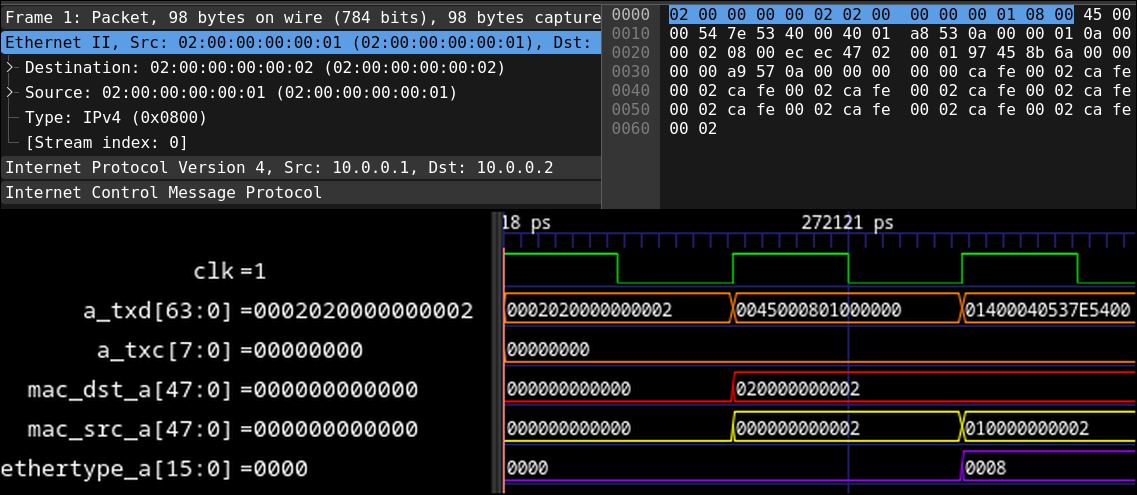
\includegraphics[width=0.94\textwidth, height=0.45\textheight, keepaspectratio]{figures/screenshot4_headers_correlation.png}}
        \vspace{1mm}
        \captionof{figure}{Cycle-by-cycle alignment between Wireshark L2/L3 hex and 64-bit lane distribution on \texttt{a\_txd[63:0]}.}
    \end{center}
\end{frame}

% ==========================================
% SLIDE 7: SW-to-HW Correlation: Payload Pattern
% ==========================================
\begin{frame}{6. SW-to-HW Correlation: Multi-Lane Payload (\texttt{0xCAFE0002})}
    \vspace{1mm}
    \textbf{ICMP Endpoints, Kernel Timestamp \& Multi-Lane Payload Streaming:}
    \begin{itemize}\scriptsize
        \item \textbf{Cycles 4--5 (IP Endpoints \& ICMP Header)}: Endpoints \texttt{10.0.0.1} $\rightarrow$ \texttt{10.0.0.2}, ICMP Type 8 Code 0 (\texttt{08 00}), Checksum \texttt{0xECEC}, and ID \texttt{0x4702}.
        \item \textbf{Cycles 6--8 (16B Timestamp \& Payload Transition)}: Kernel timestamp across Cycles 6--8, with Lanes 2--7 of Cycle 8 initiating the \texttt{ca fe 00 02} pattern (\texttt{TXD = 0xFECA0200FECA0000}).
        \item \textbf{Sustained Throughput}: Continuous 64-bit parallel transmission (8 bytes/cycle).
    \end{itemize}
    
    \vspace{1mm}
    \begin{center}
        \imageframe{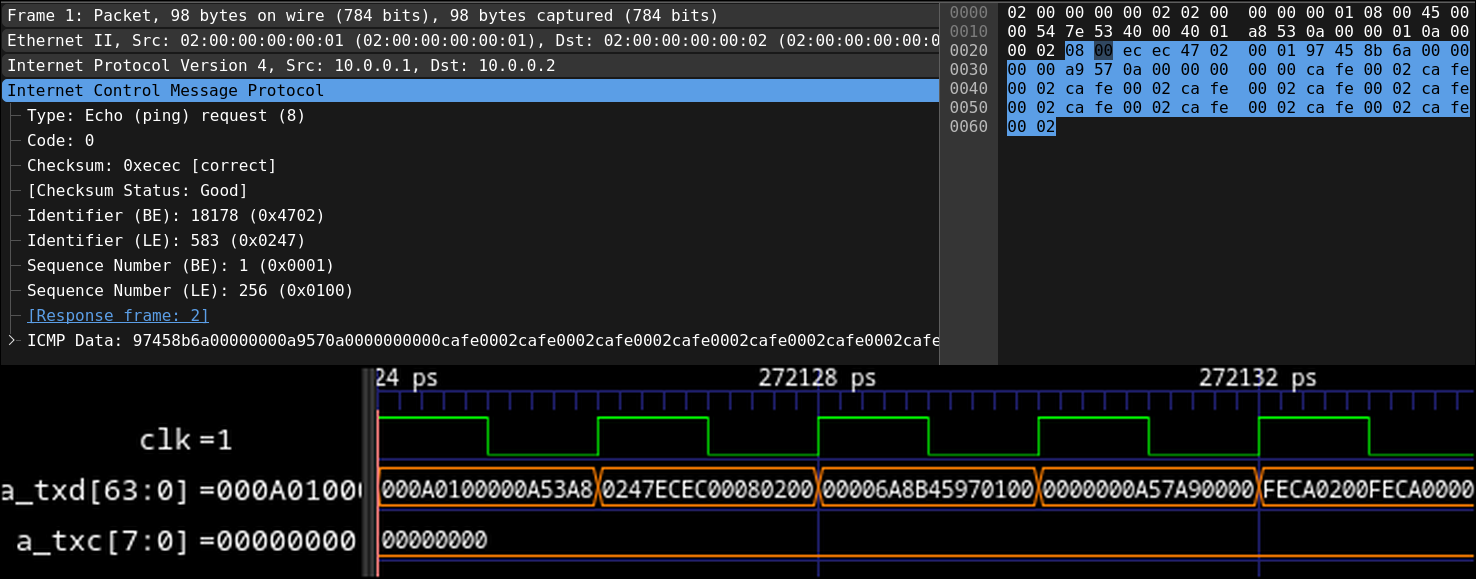
\includegraphics[width=0.94\textwidth, height=0.45\textheight, keepaspectratio]{figures/screenshot5_payload_correlation.png}}
        \vspace{1mm}
        \captionof{figure}{Multi-lane distribution of ICMP headers, timestamp, and \texttt{0xCAFE0002} payload across 64-bit XGMII cycles.}
    \end{center}
\end{frame}

% ==========================================
% SLIDE 8: Frame Termination (/T/) & FCS Validation
% ==========================================
\begin{frame}{7. Frame Termination (\texttt{/T/}) \& FCS (CRC-32) Validation}
    \vspace{1mm}
    \textbf{Frame Check Sequence (FCS) Appending \& Control Delimiter Signaling (Cycle 13):}
    \begin{itemize}\scriptsize
        \item \textbf{Data \& FCS Field (Lanes 0--5)}: Lanes 0--1 carry the final 2 payload bytes (\texttt{00 02}); Lanes 2--5 carry the 4-byte CRC-32 FCS (\texttt{0x022EE9EC}).
        \item \textbf{Control Delimiters (Lanes 6--7)}: Lane 6 asserts Terminate (\texttt{/T/ = 0xFD}, \texttt{TXC[6]=1}); Lane 7 fills with Idle (\texttt{/I/ = 0x07}, \texttt{TXC[7]=1}), setting \texttt{TXC = 8'hC0}.
    \end{itemize}
    
    \vspace{1mm}
    \begin{center}
        \imageframe{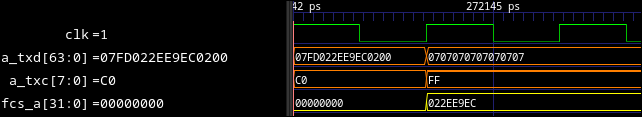
\includegraphics[width=0.94\textwidth, height=0.45\textheight, keepaspectratio]{figures/screenshot6_termination_fcs.png}}
        \vspace{1mm}
        \captionof{figure}{Cycle 13 frame termination: FCS CRC-32 (\texttt{0x022EE9EC}), and Terminate delimiter (\texttt{/T/ = 0xFD}).}
    \end{center}
\end{frame}

% ==========================================
% SLIDE 9: Pipeline Latency & Register Timing Verification
% ==========================================
\begin{frame}{8. Pipeline Latency \& Register Timing Verification}
    \vspace{1mm}
    \textbf{RTL Synchronous Registered Datapath Verification (\texttt{top.sv}):}
    \begin{itemize}\scriptsize
        \item \textbf{RTL Non-Blocking Assignment (\texttt{<=})}: Flip-flop registers in \texttt{top.sv} (\texttt{b\_rxd <= a\_txd}) use non-blocking assignments, creating the true physical 1-clock delay ($T_{\text{latency}} = 1\ T_{\text{clk}}$).
        \item \textbf{Synchronous Testbench Timing}: \texttt{wrapper.cpp} drives stimulus synchronously on \texttt{posedge clk} to accurately model SystemVerilog launch-register timing.
        \item \textbf{Deterministic 1-Cycle Latency}: Confirms exact cycle-accurate pipeline delay between TX input and RX output registers.
    \end{itemize}
    
    \vspace{1mm}
    \begin{center}
        \imageframe{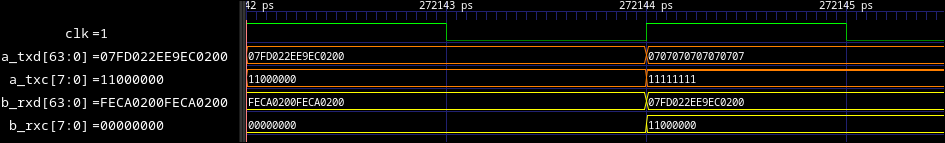
\includegraphics[width=0.94\textwidth, height=0.45\textheight, keepaspectratio]{figures/screenshot7_latency.png}}
        \vspace{1mm}
        \captionof{figure}{GTKWave trace: true 1-clock-cycle register latency ($1\ T_{\text{clk}}$) through RTL non-blocking assignments.}
    \end{center}
\end{frame}

% ==========================================
% SLIDE 10: Conclusion / Standout Slide
% ==========================================
\begin{frame}[standout]
    \Huge \textbf{Thank You!}\\[1.2em]
\end{frame}

\end{document}
